\documentclass[smaller,handout,table]{beamer}

\usetheme{clecturesty}

\subtitle{Lecture 4 of 5}

\begin{document}

{
\logo{
\includegraphics[width=0.30\textwidth]{imperialblue}}
\begin{frame}
  \titlepage
\end{frame}
}

\section{Matrices continued...}
\subsection{Last Week...}
\begin{frame}{Last Week...}
\begin{itemize}
\item A \kw{char} is the smallest addressable data type (1 byte). It is used as either an \texttt{ascii} character or a very small integer.
\item \texttt{stdin, stderr and stdout} are the standard console streams. File streams are opened with \texttt{fopen}.
\item Memory can be allocated dynamically using \texttt{malloc}. This is useful for large (or unknown size) arrays and matrices.
\item \texttt{free} is used to release previously allocated memory back to the stack; forgetting to 'free' memory causes memory-leaks.
\end{itemize}
\end{frame}


\subsection{Working with Matrices}
\begin{frame}
\frametitle{Matrices - Details}
\framesubtitle{For matrices allocated in the previous lecture}
\begin{tabular}{l l}
\tt matrix & points to a matrix \textit{- more specifically, it points to}
\\&\textit{an array holding the addresses of each row}\\
\tt matrix[0]& points to the first row of the matrix\\
\tt matrix[0][0]&The top left element of the matrix
\end{tabular}\\
\vspace{0.2in}
Which have the following types:\\
\begin{tabular}{l l}
\tt matrix& \tt \kw{double} **\\
\tt matrix[0]&\tt \kw{double} *\\
\tt matrix[0][0]& \tt \kw{double}
\end{tabular}
\end{frame}

\subsection{Higher Dimension Arrays}
\begin{frame}[fragile]
\frametitle{Higher Dimensional Arrays}
\begin{semiverbatim}
\tiny
\kr\kl\kw{double} *** alloc3Tensor(\kw{unsigned int} dim)
\kl\{
\kl   \kw{unsigned int} i, j;
\kl   \kw{double} *** tensor;
\kl   tensor = (\kw{double} ***) malloc(dim*\kw{sizeof}(\kw{double} **));
\kl   \kw{if} (!tensor) \kw{return} NULL;
\kl   tensor[0] = (\kw{double} **) malloc(dim*dim*\kw{sizeof}(\kw{double} *));
\kl   \kw{if} (!tensor[0])
\kl   \{
\kl      free(tensor);
\kl      \kw{return} NULL;
\kl   \}
\kl   tensor[0][0] = (\kw{double} *) malloc(dim*dim*dim*\kw{sizeof}(\kw{double}));
\kl   \kw{if} (!tensor[0][0])
\kl   \{
\kl      free(tensor[0]); free(tensor);
\kl      \kw{return} NULL;
\kl   \}
\kl   \kw{for} (i = 1; i < dim; i++)
\kl      tensor[0][i] = tensor[0][i-1]+dim;
\kl   \kw{for} (i = 1; i < dim; i++)
\kl   \{
\kl      tensor[i] = tensor[i-1] + dim;
\kl      tensor[i][0] = tensor[i-1][0] + dim * dim;
\kl      \kw{for} (j = 1; j < dim; j++)
\kl         tensor[i][j] = tensor[i][j-1] + dim;
\kl   \}
\kl   \kw{return} tensor;
\kl\}
\end{semiverbatim}
\end{frame}

\begin{frame}[fragile]
\frametitle{More Multi-Index}
\begin{itemize}
\item The 3D array behaves as expected:\\
\begin{center}
\tt tensor[i][j][k] = 0.5;
\end{center}
\item The array can be freed with:
\begin{semiverbatim}
\kw{void} free3Tensor(\kw{double} *** tensor)
\{
   free(tensor[0][0]);
   free(tensor[0]);
   free(tensor);
\}
\end{semiverbatim}
\end{itemize}
\end{frame}

\subsection{Non-'Square' Arrays}
\begin{frame}
\frametitle{More Elaborate Data Structures}
\begin{itemize}
\item In C we are able to manipulate data directly, this has allowed us to partition a contiguous array of memory into matrix rows.
\item We needn't restrict ourselves to structures where the number of elements per row is constant, one example is Pascal's triangle:\\
\begin{center}
\tt1\\\tt1 1\\\tt1  2  1\\\tt1  3  3  1\\\tt1  4  6  4  1\\$\vdots$
\end{center}
\end{itemize}
\end{frame}

\begin{frame}[fragile]
\begin{semiverbatim}
\scriptsize
\kr\kl\kw{int} main()
\kl\{
\kl   \kw{unsigned int} size = 10, r, c;
\kl   \kw{int} ** pasc;
\kl   pasc = (\kw{int} **) malloc(size*\kw{sizeof}(\kw{int} *));
\kl   pasc[0] = (\kw{int} *) malloc(size*(size+1)*\kw{sizeof}(\kw{int})/2);
\kl   \kc{/* check the mallocs */}
\kl   \kw{for} (r=1; r < size; r++) pasc[r] = pasc[r-1]+r;
\kl   pasc[0][0] = 1;
\kl   \kw{for} (r = 1; r < size; r++)
\kl   \{
\kl      \kw{for} (c = 1; c < r; c++)
\kl         pasc[r][c] = pasc[r-1][c-1]+pasc[r-1][c];
\kl      pasc[r][0] = 1; pasc[r][r] = 1;
\kl   \}
\kl   \kw{for} (r=0; r < size; r++)
\kl   \{
\kl      \kw{for} (c = 0; c < r+1; c++)
\kl         printf(\kt{"\%3d "}, pasc[r][c]);
\kl      printf(\kt{"\\n"});
\kl   \}
\kl   free(pasc[0]);
\kl   free(pasc);
\kl   \kw{return} 0;
\kl\}
\end{semiverbatim}
\end{frame}

\begin{frame}[fragile]
\frametitle{Pascal's Triangle}
\begin{itemize}
\item The program outputs:
\vspace{-0.2in}
\begin{semiverbatim}
\small
  1
  1   1
  1   2   1
  1   3   3   1
  1   4   6   4   1
  1   5  10  10   5   1
  1   6  15  20  15   6   1
  1   7  21  35  35  21   7   1
  1   8  28  56  70  56  28   8   1
  1   9  36  84 126 126  84  36   9   1
\end{semiverbatim}
\item Whilst in memory, the data structure looks like:
\begin{tabular}{|c|c|c|c|c|c|c|c|c|c|c|}
\hline
\tt1&\tt1&\tt1&\tt1&\tt2&\tt1&\tt1&\tt3&\tt3&\tt1&$\cdots$\\
\hline
\end{tabular}
\end{itemize}
\end{frame}

\section{Structs}
\subsection{Custom Data Types}
\begin{frame}[fragile]
\frametitle{Custom Data Types}
Recall, when dealing with files we used:
\begin{semiverbatim}
FILE * file;
file = fopen (\kt{"myfile.txt"}, \kt{"r"});
\end{semiverbatim}
{\tt FILE} is in fact a custom data type, with its own size:
\begin{semiverbatim}
\kw{\#include} \kt{<stdio.h>}

\kw{int} main()
\{
   printf(\kt{"sizeof(FILE) = \%d\\n"}, \kw{sizeof}(FILE));
   \kw{return} 0;
\}
\end{semiverbatim}
\end{frame}

\begin{frame}[fragile]
\frametitle{Except from MS - \kt{\tt <stdio.h>}}
(From Visual Studio 2008)
\begin{semiverbatim}
\kw{struct} _iobuf \{
   \kw{char} *_ptr;
   \kw{int}   _cnt;
   \kw{char} *_base;
   \kw{int}   _flag;
   \kw{int}   _file;
   \kw{int}   _charbuf;
   \kw{int}   _bufsiz;
   \kw{char} *_tmpfname;
   \};
\kw{typedef struct} _iobuf FILE;
\end{semiverbatim}
\end{frame}

\subsection{Defining Our Structs}
\begin{frame}[fragile]
\frametitle{{\tt typedef} Structures : Custom Data Types}
\begin{itemize}
\item {\tt FILE} is a custom data type defined in \kt{\tt <stdio.h>}.
\item It is comprised of elements of different, known, types.
\item Each element of the {\tt FILE} \emph{structure} has its own name.
\end{itemize}

Let's consider a structure of our own, one of the simplest examples is a complex number:
\begin{columns}
\begin{column}{5cm}
\begin{semiverbatim}
\kw{typedef struct}
\{
   \kw{double} real;
   \kw{double} imag;
\} complex;
\end{semiverbatim}
\end{column}
\begin{column}{5cm}
\begin{alertblock}{C99}
C99 fully supports its own {\tt \_Complex}
type.
\end{alertblock}
\end{column}
\end{columns}
\end{frame}

\begin{frame}[fragile]
\frametitle{{\tt typedef} Structures - II}
Definitions of structures take the following form:
\begin{semiverbatim}
   \kw{typedef struct}
   \{
      \emph{elementType} \emph{elementName};
      \emph{elementType} \emph{elementName};
      \vdots
   \} \emph{structureTypeName} ;
\end{semiverbatim}
\end{frame}

\subsection{Using Structures}
\begin{frame}
\frametitle{Handling Structures}
\begin{enumerate}
\item A structure may be an argument to a function.
\item A function may return a structure.
\item A pointer may point to a structure.
\item Structures are referenced as normal: {\tt \&name}.
\item Elements of a structure are referenced as: {\tt \&name.element}.
\item A pointer to a structure may be passed to a function.
\item If {\tt p} is a pointer to a structure, then {\tt p->member} allows us to access it's members.
\end{enumerate}
\end{frame}

\begin{frame}[fragile]
\frametitle{Example Function Applying to Structures}
\vspace{-0.2in}
\begin{semiverbatim}
\scriptsize
\kr\kl\kw{\#include} \kt{<stdio.h>}
\kl
\kl\kw{typedef struct}
\kl\{
\kl   \kw{double} real;
\kl   \kw{double} imag;
\kl\} complex;
\kl
\kl\kw{void} printComplex(complex * mc)
\kl\{
\kl   printf(\kt{"\%lg + \%lgi\\n"}, mc->real, mc->imag);
\kl\}
\kl
\kl\kw{int} main()
\kl\{
\kl   complex c1 = \{1.0, 0.5\}; \kc{/* assignment at declaration */}
\kl   printComplex(&c1);       \kc{/* pass pointer to struct */}
\kl   c1.real = 10.0;          \kc{/* piecewise assignment */}
\kl   printComplex(&c1);
\kl   \kw{return} 0;
\kl\}
\end{semiverbatim}
\end{frame}

\begin{frame}
\frametitle{More Structures}
\begin{itemize}
\item Passing structures via pointer is usually more efficient.
\item Assignment can be done at declaration or after.
\item In C we are not allowed to overload operators, so the following won't work:
\begin{center}
{\tt c1 = c2 + c3;} (where {\tt c1} and {\tt c2} are {\tt complex})
\end{center}
so we need to do something like:
\begin{center}
{\tt complexAdd(\&c1, \&c2, \&c3);}
\end{center}
\item Arrays of {\tt \kw{struct}}s are allowed (so matrices can consist of complex numbers for example).
\item Structures can contain structures as elements.
\end{itemize}
\end{frame}

\subsection{A Note on Complex Numbers}
\begin{frame}
\frametitle{Complex Number Support in C/C++}
\begin{exampleblock}{C++}
Complex numbers are supported in C++ as {\tt \kw{class}}es, also the operators are overloaded properly too meaning any code which uses them will be concise.
(look in {\tt \kt{<complex>}}).
\end{exampleblock}

\begin{block}{C99}
Complex numbers are supported as a native data type (not {\tt \kw{struct}}) in C99. Unfortunately not many compilers support this. GNU C, fully supports complex numbers (see {\tt \kt{<complex.h>}}).
\end{block}

\begin{alertblock}{C90}
Complex number support in C90 is non-existent. I would recommend either third party libraries or a switch to C99/C++ for heavy complex number use.
\end{alertblock}
\end{frame}


\section{More on Scope}
\subsection{Scope Blocks}
\begin{frame}[fragile]
\frametitle{Scope Blocks}
\begin{small}
{
Variable scope is not restricted to functions, indeed anything contained in braces (\emph{scope blocks}) has it's own scope:
\vspace{-0.1in}
\begin{semiverbatim}
\kr\kl\kw{\#include} \kt{<stdio.h>}
\kl
\kl\kw{int} main()
\kl\{
\kl   \kw{int} i = 1;
\kl
\kl   \kw{if} (i==1)
\kl   \{
\kl      \kw{int} j = 10; \kc{/* local to if block */}
\kl      printf(\kt{"i+j=\%d\\n"}, i+j);
\kl   \}
\kl
\kl   \kc{/* printf("j = \%d\\n", j); - error */}
\kl
\kl   \kw{return} 0;
\kl\}
\end{semiverbatim}
}
\end{small}
\end{frame}

\subsection{The Lifetime of a Variable}
\begin{frame}[fragile]
\frametitle{Local Variable Lifetime}
The lifetime of a local variable is limited:
\begin{semiverbatim}
\kw{\#include} \kt{<stdio.h>}

\kw{void} F1()
\{
   \kw{int} i = 1;
   printf(\kt{"In F1(): i = \%d\\n"}, i);
   i = i + 1; \kc{/* won't do much */}
\}

\kw{int} main()
\{
   F1();
   F1();
   \kw{return} 0;
\}
\end{semiverbatim}
\end{frame}

\begin{frame}
\frametitle{Local Variables}
\begin{itemize}
\item Every time {\tt F1()} is invoked, the value of {\tt i} is reset to 1.
\item The variable {\tt i} is a local variable which lives on the stack:
\begin{itemize}
\item it will be destroyed every time we leave {\tt F1()},
\item and recreated every time we invoke {\tt F1()}.
\end{itemize}
\item We can ask the C compiler to retain the value of {\tt i}:
\begin{block}{{\tt static} variables}
A variable can be declared to be \kw{\tt static}, this tells the C compiler to set aside memory other than the stack to store the variable. The variable will not be destroyed until the program ends.
\end{block}
\end{itemize}
\end{frame}

\subsection{Static and Global Variables}
\begin{frame}
\frametitle{Why Use Static Variables?}
\begin{itemize}
\item To count the number of times a function has been called.
\item To have the function remember something between calls so on subsequent calls it can calculate what has changed (time, storage, the date, etc...), or resume from where it left off (reading from a list...)
\end{itemize}

\begin{exampleblock}{Worked Example: Elapsed Time}
\begin{itemize}
\item We write a function {\tt timer} which returns the time since it was last called.
\item Our program will contain two {\tt .c} files to demonstrate linking.
\end{itemize}
\end{exampleblock}
\end{frame}

\begin{frame}[fragile]
\frametitle{Timer Example: {\tt timer()}}
\begin{semiverbatim}
\kr\kl\kw{\#include} \kt{<time.h>} \kc{/* for clock function */}
\kl
\kl\kw{double} timer()
\kl\{
\kl   \kw{static double} oldTime = 0.0;
\kl   \kw{double} newTime, diff;
\kl
\kl   newTime = clock();
\kl   diff = newTime - oldTime;
\kl   oldTime = newTime;
\kl   \kw{return} diff/CLOCKS_PER_SEC;
\kl\}
\end{semiverbatim}
\end{frame}

\begin{frame}[fragile]
\frametitle{Timer Example: {\tt main()}}
\begin{semiverbatim}
\small
\kr\kl\kw{\#include} \kt{<stdio.h>}
\kl
\kl\kw{double} timer(); \kc{/* declare timer */}
\kl
\kl\kw{int} main()
\kl\{
\kl   timer(); \kc{/* reset clock */}
\kl   printf(\kt{"Wait... and hit return\\n"});
\kl   getchar(); \kc{/* wait for return */}
\kl   printf(\kt{"Elapsed time: \%.2f seconds\\n"}, timer());
\kl   printf(\kt{"Resetting clock, hit enter again\\n"});
\kl   getchar();
\kl   printf(\kt{"Elapsed time: \%.2f seconds\\n"}, timer());
\kl   \kw{return} 0;
\kl\}
\end{semiverbatim}
\end{frame}

\begin{frame}[fragile]
\frametitle{Global Variables - Shared between Functions}
We can define a \emph{global} variable:
\begin{semiverbatim}
\small
\kr\kl\kw{\#include} \kt{<stdio.h>}
\kl
\kl\kw{double} global = 42.0;
\kl
\kl\kw{void} F1()
\kl\{
\kl   printf(\kt{"Global = \%g\\n"}, global);
\kl\}
\kl
\kl\kw{int} main()
\kl\{
\kl   F1();
\kl   global = global + 1.0;
\kl   F1();
\kl   \kw{return} 0;
\kl\}
\end{semiverbatim}
\end{frame}

\begin{frame}
\frametitle{Global Variables - Between Multiple Files}
\begin{exampleblock}{Global to All Files}
If we want to share a global variable between files,
then we define it \emph{once} as:\\
{\tt type myglobalvariable = value;}\\
Then in every other file we declare it as:\\
{\tt \kw{extern} type myglobalvariable;}
\end{exampleblock}

\begin{alertblock}{Global Only to Current File}
If we do not wish to share a global variable, we
define it as follows:\\
{\tt \kw{static} type myPrivateGlobal = value;}
\end{alertblock}
\end{frame}

\begin{frame}[fragile]
\frametitle{Shared/Private Global Variables - File 1 of 2}
\begin{semiverbatim}
\footnotesize
\kr\kl\kw{\#include} \kt{<stdio.h>}
\kl
\kl\kw{int} globalEverywhere = 42;
\kl\kw{static int} globalHereOnly = 1;
\kl
\kl\kw{void} F2(); \kc{/* defined in file 2 */}
\kl
\kl\kw{int} main()
\kl\{
\kl   printf(\kt{"globalEverywhere = \%d\\n"}, globalEverywhere);
\kl   printf(\kt{"globalHereOnly = \%d\\n"}, globalHereOnly);
\kl
\kl   F2();
\kl
\kl   printf(\kt{"globalEverywhere = \%d\\n"}, globalEverywhere);
\kl   printf(\kt{"globalHereOnly = \%d\\n"}, globalHereOnly);
\kl
\kl   \kw{return} 0;
\kl\}
\end{semiverbatim}
\end{frame}

\begin{frame}[fragile]
\frametitle{Shared/Private Global Variables - File 2 of 2}
\vspace{-0.1in}
\begin{semiverbatim}
\small
\kr\kl\kw{\#include} \kt{<stdio.h>}
\kl
\kl\kw{extern int} globalEverywhere;
\kl\kc{/*if we forget the extern we get a linker error */}
\kl
\kl\kw{static int} globalHereOnly = 100;
\kl
\kl\kw{void} F2()
\kl\{
\kl   printf(\kt{"F2(): globalEverywhere = \%d\\n"},
\kl                 globalEverywhere);
\kl                 
\kl   printf(\kt{"F2(): globalHereOnly = \%d\\n"},
\kl                 globalHereOnly);
\kl\}
\end{semiverbatim}
\end{frame}

\section{Compiling}
\subsection{Compilation of C}
\begin{frame}
\frametitle{Compilation}
\begin{itemize}
\item As seen in the first lecture, C programs are \emph{compiled} into a low level (machine specific language).
\item This language is called \emph{assembly language}.
\item Most C compilers allow you to view the assembler that they generate.
\end{itemize}
\end{frame}

\begin{frame}[fragile]
\frametitle{{\tt addMatrices} revisited - C code}
From the last lecture we saw a function to add two matrices together:
\begin{semiverbatim}
\small
\kw{void} addMatrices(\kw{double} ** matrixA, \kw{double} ** matrixB,
                 \kw{double} ** matrixR,
                 \kw{unsigned int} rows, \kw{unsigned int} cols)
\{
   \kw{unsigned int} i, j;
   \kw{for} (i = 0; i < rows; i++)
      \kw{for} (j = 0; j < cols; j++)
         matrixR[i][j] = matrixA[i][j]+matrixB[i][j];
\}
\end{semiverbatim}
When we compile this, we get...
\end{frame}

\begin{frame}[fragile]
\frametitle{{\tt addMatrices} revisited - when compiled...}
\begin{columns}
\begin{column}{5cm}
\vspace{-0.2in}
\begin{semiverbatim}
\tiny
\_addMatrices PROC
; 35   : \{
        push    ebp
        mov     ebp, esp
        sub     esp, 216
        push    ebx
        push    esi
        push    edi
        lea     edi, DWORD PTR [ebp-216]
        mov     ecx, 54
        mov     eax, -858993460
        rep stosd
; 36   :        unsigned int i, j;
; 37   :        for (i = 0; i < rows; i++)
        mov     DWORD PTR \_i\$[ebp], 0
        jmp     SHORT \$LN6@addMatrice
\$LN5@addMatrice:
        mov     eax, DWORD PTR \_i\$[ebp]
        add     eax, 1
        mov     DWORD PTR \_i\$[ebp], eax
\$LN6@addMatrice:
        mov     eax, DWORD PTR \_i\$[ebp]
        cmp     eax, DWORD PTR \_rows\$[ebp]
        jae     SHORT \$LN4@addMatrice
; for (j = 0; j < cols; j++)
        mov     DWORD PTR \_j\$[ebp], 0
        jmp     SHORT \$LN3@addMatrice
\$LN2@addMatrice:
        mov     eax, DWORD PTR \_j\$[ebp]
        add     eax, 1
        mov     DWORD PTR \_j\$[ebp], eax
\end{semiverbatim}
\end{column}
\begin{column}{5cm}
\vspace{-0.2in}
\begin{semiverbatim}
\tiny
\$LN3@addMatrice:
        mov     eax, DWORD PTR \_j\$[ebp]
        cmp     eax, DWORD PTR \_cols\$[ebp]
        jae     SHORT \$LN1@addMatrice
;matrixR[i][j] = matrixA[i][j]+matrixB[i][j];
        mov     eax, DWORD PTR \_i\$[ebp]
        mov     ecx, DWORD PTR \_matrixA\$[ebp]
        mov     edx, DWORD PTR [ecx+eax*4]
        mov     eax, DWORD PTR \_i\$[ebp]
        mov     ecx, DWORD PTR \_matrixB\$[ebp]
        mov     eax, DWORD PTR [ecx+eax*4]
        mov     ecx, DWORD PTR \_j\$[ebp]
        mov     esi, DWORD PTR \_j\$[ebp]
\textcolor{red}{        fld     QWORD PTR [edx+ecx*8]}
\textcolor{red}{        fadd    QWORD PTR [eax+esi*8]}
        mov     edx, DWORD PTR \_i\$[ebp]
        mov     eax, DWORD PTR \_matrixR\$[ebp]
        mov     ecx, DWORD PTR [eax+edx*4]
        mov     edx, DWORD PTR \_j\$[ebp]
\textcolor{red}{        fstp    QWORD PTR [ecx+edx*8]}
        jmp     SHORT \$LN2@addMatrice
\$LN1@addMatrice:
        jmp     SHORT \$LN5@addMatrice
\$LN4@addMatrice:
        pop     edi
        pop     esi
        pop     ebx
        mov     esp, ebp
        pop     ebp
        ret     0
\_addMatrices ENDP
\end{semiverbatim}
\end{column}
\end{columns}
\end{frame}

\subsection{Optimisation}
\begin{frame}
\frametitle{Optimisation}
\begin{itemize}
\item A few lines of C becomes $>30$ lines of assembler (only three of which are actually floating point instructions!).
\item It is possible to write a much smaller assembler routine by hand $\approx$10-20 instructions long.
\item This would run $\approx$3 times quicker than the C compiled routine (this is a general rule of thumb).
\item Any custom assembly code would only target a very specific chip, however.
\end{itemize}
\end{frame}

\begin{frame}
\frametitle{Optimisation II}
\begin{itemize}
\item Rather than rewrite the assembly code, it is easier to ask the C compiler to perform code optimisation itself.
\item By default C will compile the code as it appears (the exact order of operations is preserved etc), this aids debugging.
\item C compilers can be told to optimise their code in the following ways:
\begin{center}
\begin{tabular}{l p{220pt}}
MSVC&Project configuration options can be set, defaults in ``Release'' build do a good job.\\
gcc&The {\tt -O} command line flags influence optimisation, {\tt -O0} means ``off'' whilst {\tt -O3} means ``extremely aggressive''.
\end{tabular}
\end{center}
\end{itemize}
\end{frame}

\begin{frame}[fragile]
\frametitle{Optimisation Example - Visual Studio 2008}
\begin{columns}
\begin{column}{5cm}
\begin{center}
Debug Build
\end{center}
\begin{semiverbatim}
\tiny
\$LN2@addMatrice:
        mov     eax, DWORD PTR \_j\$[ebp]
        add     eax, 1
        mov     DWORD PTR \_j\$[ebp], eax
\$LN3@addMatrice:
        mov     eax, DWORD PTR \_j\$[ebp]
        cmp     eax, DWORD PTR \_cols\$[ebp]
        jae     SHORT \$LN1@addMatrice
;matrixR[i][j] = matrixA[i][j]+matrixB[i][j];
        mov     eax, DWORD PTR \_i\$[ebp]
        mov     ecx, DWORD PTR \_matrixA\$[ebp]
        mov     edx, DWORD PTR [ecx+eax*4]
        mov     eax, DWORD PTR \_i\$[ebp]
        mov     ecx, DWORD PTR \_matrixB\$[ebp]
        mov     eax, DWORD PTR [ecx+eax*4]
        mov     ecx, DWORD PTR \_j\$[ebp]
        mov     esi, DWORD PTR \_j\$[ebp]
\textcolor{red}{        fld     QWORD PTR [edx+ecx*8]}
\textcolor{red}{        fadd    QWORD PTR [eax+esi*8]}
        mov     edx, DWORD PTR \_i\$[ebp]
        mov     eax, DWORD PTR \_matrixR\$[ebp]
        mov     ecx, DWORD PTR [eax+edx*4]
        mov     edx, DWORD PTR \_j\$[ebp]
\textcolor{red}{        fstp    QWORD PTR [ecx+edx*8]}
        jmp     SHORT \$LN2@addMatrice
\end{semiverbatim}
\end{column}
\begin{column}{5cm}
\begin{center}
Release Build
\end{center}
\begin{semiverbatim}
\tiny
;matrixR[i][j] = matrixA[i][j]+matrixB[i][j];
\textcolor{red}{                fld     QWORD PTR [edx+eax]}
\textcolor{red}{                fadd    QWORD PTR [eax]}
\textcolor{red}{                fstp    QWORD PTR [esi+eax]}
        add     eax, 8
        dec     ebx
        jne     SHORT \$LL3@addMatrice
\end{semiverbatim}
\vspace{1.55in}
\end{column}
\end{columns}
\end{frame}

\section{Using Binary Data}
\subsection{Efficient Data Packing}
\begin{frame}
\frametitle{Bits and Bytes}
\begin{columns}
\begin{column}{5cm}
\begin{block}{Bytes}
Smallest \emph{addressable} unit of memory, each byte is composed of eight bits.
\end{block}
\end{column}
\begin{column}{5cm}
\begin{block}{Bits}
These are the smallest units of computer memory, each bit can be either 0 or 1.
\end{block}
\end{column}
\end{columns}
\vspace{0.2in}
\begin{itemize}
\item Addressing bits individually requires some extra operations to be carried out.
\item There are good reasons for accessing data at the bit-level however.
\end{itemize}
\end{frame}

\begin{frame}
\frametitle{Efficient Data Packing}
\begin{block}{Given a 32 million base pair chromosome}
\begin{tabular}{l l}
It will require: &$\approx$128 megabytes to store as {\tt int}\\
&$\approx$32 megabytes to store as {\tt char}\\
&$\approx$8 megabytes to store as bit data.
\end{tabular}
\end{block}
\begin{block}{Computer Graphics}
Given a monochrome print image of 2400 dpi rendered over 80 square inches gives $\approx 500,000,000$ dots. This takes up:
\begin{center}
\begin{tabular}{l}
$\approx$1 gigabyte if using {\tt short}\\
$\approx$64 megabytes if using bits.
\end{tabular}
\end{center}
\end{block}
\end{frame}

\subsection{Unsigned Integers}
\begin{frame}
\frametitle{Bit Manipulation Friendly Data Types}
As seen before, the unsigned integer data types have values ranging from 0 to $2^n-1$ where $n$ is the number of bits in the data type:
\begin{center}
\rowcolors[]{1}{blue!20}{blue!10}
\begin{tabular}{l c}
\bf Data Type&\bf$n$\\
\tt unsigned short&16\\
\tt unsigned int&32\\
\tt unsigned long int&32\\
\tt unsigned long long int&64\\
\end{tabular}
\end{center}
\textit{(Unsigned data types are also desirable for accessing array indices as they can never be negative.)}\\
When using these data types for bit data we ignore the resulting value it stores and instead just focus on the $n$ zeros or ones in the data type.
\end{frame}

\begin{frame}
\frametitle{How to Get Them In and Out of The Computer}
\begin{itemize}
\item They can be read using {\tt scanf} and {\tt \kt{"\%u"}}, {\tt \kt{"\%lu"}}
 or {\tt \kt{"\%Lu"}}.
\item They can be printed using {\tt printf} and {\tt \kt{"\%u"}} or {\tt \kt{"\%Lu"}}.
\item We can output to octal (base 8 numbers) using {\tt printf} and {\tt \kt{"\%o"}}
\item Also we can output to hexadecimal (base 16: 0-9 and a-f) using {\tt printf} and {\tt \kt{"\%x"}} or {\tt \kt{"\%X"}}.
\end{itemize}
\begin{block}{Example - byte ({\tt char})}
\begin{tabular}{l l}
Binary&\tt10101011\\
Hexadecimal&\tt AB\\
Decimal&\tt171\\
Octal&\tt253
\end{tabular}
\end{block}
\end{frame}

\subsection{Manipulating Bits}
\begin{frame}
\frametitle{Manipulating Bits within an Unsigned Integer}
\begin{itemize}
\item C can shift all the bits comprising a number a fixed number of places to the left or right.
\item Zeros are propagated in to the vacated spaces.
\item Bits that shift outside, disappear. (i.e. the shift is not cyclic).
\item Bit shifting is accomplished with the {\tt >>} (right) and {\tt <<} (left) operators.
\end{itemize}
For example:
\begin{center}
\tt 1 << 2 = 4\\
\tt 8 >> 3 = 1
\end{center}
\begin{block}{}
Bit shifts are much cheaper than multiplying or dividing by powers of two.
\end{block}
\end{frame}

\begin{frame}
\frametitle{4 Bitwise operators {\tt \&}, {\tt|}, {\tt$\wedge$} and {\tt$\sim$}}
Assuming 0 is false and 1 is true, we have the following bitwise logical operators.
\begin{columns}
\begin{column}{5cm}
\begin{block}{And Operator(\&)}
\begin{tabular}{r|c c c c}
N1&0&0&1&1\\
N2&0&1&0&1\\
\hline
N1 \& N2&0&0&0&1
\end{tabular}
\end{block}

\begin{block}{Exclusive Or({\tt$\wedge$})}
\begin{tabular}{r|c c c c}
N1&0&0&1&1\\
N2&0&1&0&1\\
\hline
N1 {\tt$\wedge$} N2&0&1&1&0
\end{tabular}
\end{block}

\end{column}
\begin{column}{5cm}
\begin{block}{Or Operator({\tt|})}
\begin{tabular}{r|c c c c}
N1&0&0&1&1\\
N2&0&1&0&1\\
\hline
N1 {\tt|} N2&0&1&1&1
\end{tabular}
\end{block}

\begin{block}{Not Operator({\tt$\sim$})}
\begin{tabular}{r|c c}
N1&0&1\\
\hline
{\tt$\sim$}N1&1&0
\end{tabular}
\end{block}
\vspace{0.13in}
\end{column}
\end{columns}
\end{frame}

\subsection{Case Study: The Sieve of Eratosthenes}
\begin{frame}{Case Study: The Sieve of Eratosthenes}

\begin{block}{Algorithm}
List all odd numbers up to $n$. Then, starting at the beginning of the list$\ldots$
\begin{enumerate}
\item select next available number in the list, $i$, as prime
\item if $i \le \sqrt{n}$ remove all multiples of $i$ in the list greater than $i^2$
\item repeat$\ldots$
\end{enumerate}
We prepend $2$ to this list, making it the list of primes $< n$.
\end{block}
\end{frame}

\begin{frame}{The Sieve of Eratosthenes: Algorithm Example}
For $n = 51$:\\
Write out list of odd numbers
\begin{center}
\kpr
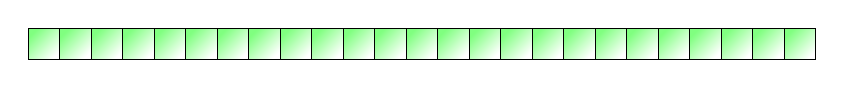
\begin{tikzpicture}[]
\foreach \x in {0.0, 0.4, ..., 9.6}
   \shadedraw [top color=green!50,shading angle=45] (\x,0) rectangle +(0.4,0.4);
\foreach \x in {0.2, 0.6, ..., 10.2}
   \node at (\x, 0.2) {{\scriptsize\kp}};  
\end{tikzpicture}
\end{center}
Select, and remove multiples of, $3$
\begin{center}
\kpr
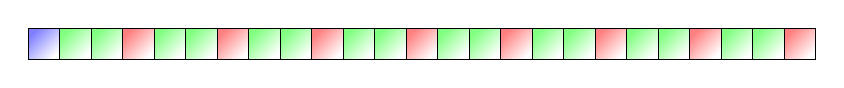
\begin{tikzpicture}[]
\foreach \x in {0.0, 0.4, ..., 9.6}
   \shadedraw [top color=green!50,shading angle=45] (\x,0) rectangle +(0.4,0.4); \shadedraw [top color=blue!50, shading angle=45] (0, 0) rectangle +(0.4,0.4);
\foreach \x in {1.2, 2.4, ..., 9.6}
   \shadedraw [top color=red!50,shading angle=45] (\x,0) rectangle +(0.4,0.4); \foreach \x in {0.2, 0.6, ..., 10.2}
   \node at (\x, 0.2) {{\scriptsize\kp}};  
\end{tikzpicture}
\end{center}
Select, and remove multiples of, $5$
\begin{center}
\kpr
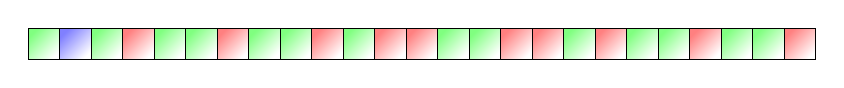
\begin{tikzpicture}[]
\foreach \x in {0.0, 0.4, ..., 9.6}
   \shadedraw [top color=green!50,shading angle=45] (\x,0) rectangle +(0.4,0.4); \shadedraw [top color=blue!50, shading angle=45] (0.4,0) rectangle +(0.4,0.4);
\foreach \x in {1.2, 2.4, ..., 9.6}
   \shadedraw [top color=red!50,shading angle=45] (\x,0) rectangle +(0.4,0.4);
\foreach \x in {2.4, 4.4, ..., 9.6}
   \shadedraw [top color=red!50,shading angle=45] (\x,0) rectangle +(0.4,0.4);
\foreach \x in {0.2, 0.6, ..., 10.2}
   \node at (\x, 0.2) {{\scriptsize\kp}};  
\end{tikzpicture}
\end{center}
Select, and remove the multiple of, $7$
\begin{center}
\kpr
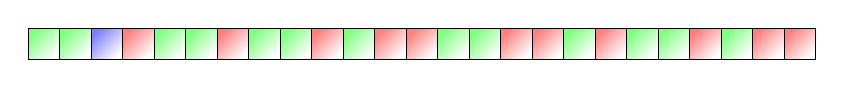
\begin{tikzpicture}[]
\foreach \x in {0.0, 0.4, ..., 9.6}
   \shadedraw [top color=green!50,shading angle=45] (\x,0) rectangle +(0.4,0.4); \shadedraw [top color=blue!50, shading angle=45] (0.8,0) rectangle +(0.4,0.4);
\foreach \x in {1.2, 2.4, ..., 9.6}
   \shadedraw [top color=red!50,shading angle=45] (\x,0) rectangle +(0.4,0.4);
\foreach \x in {2.4, 4.4, ..., 9.6}
   \shadedraw [top color=red!50,shading angle=45] (\x,0) rectangle +(0.4,0.4);
\foreach \x in {3.6, 6.4, ..., 9.6}
   \shadedraw [top color=red!50,shading angle=45] (\x,0) rectangle +(0.4,0.4); \foreach \x in {0.2, 0.6, ..., 10.2}
   \node at (\x, 0.2) {{\scriptsize\kp}};  
\end{tikzpicture}
\end{center}

Select the remaining numbers and prepend $2$. This gives the primes:
\resizebox{\textwidth}{!}{
\begin{tabular}{ccccccccccccccc}
2&3&5&7&11&13&17&19&23&29&31&37&41&43&47
\end{tabular}}
\end{frame}

\begin{frame}
\frametitle{The Sieve of Eratosthenes: In C}
\begin{itemize}
\item When implementing this in C it makes sense to use a bit to indicate `primeness' of a number.
\item The smallest addressable unit of memory in C is the {\tt \kw{char}} which consists of 8 bits.
\item We therefore need to perform \emph{masking} to isolate individual bits.
\end{itemize}
\begin{block}{Masking}
We access the $i^\mathrm{th}$ bit of a variable {\tt x} as follows:
\begin{center}
\begin{tabular}{l l}
\tt \kw{if}(x \& (1 << i))& Check to see if it's set\\
\tt x |= (1 << i)& To set the bit\\
\tt x \&= $\sim$(1 << i)& To clear the bit
\end{tabular}
\end{center}
\end{block}
\end{frame}

\begin{frame}[fragile]
\frametitle{The Sieve of Eratosthenes: Implementation}
\vspace{-0.2in}
\begin{semiverbatim}
\scriptsize
\kr\kl\kw{void} findPrimes(\kw{char} * Prime\_List, \kw{int} max\_num)
\kl\{
\kl   \kw{int} current\_num, sqmax\_num;
\kl   \kw{char} Mask=1;
\kl   sqmax\_num = sqrt((float)max\_num);
\kl
\kl   \kw{for}(current\_num = 3; current\_num <= sqmax\_num; current\_num += 2)
\kl   \{
\kl      \kw{int} Pnum = current\_num / 16; \kc{/*Find which char we are on*/}
\kl      \kw{short} Pbit = (current\_num - Pnum * 16) / 2; \kc{/*Which bit in char*/}
\kl
\kl      if(~Prime\_List[Pnum] \& (Mask << Pbit))
\kl      \{   \kc{/*if the current bit in the current char is a zero(prime)}
\kl         \kc{* then lets strike out some multiples*/}
\kl         \kw{int} strike;
\kl         for(strike = current\_num * current\_num; strike <= max\_num; strike += 2 * current\_num)
\kl         \{
\kl            \kw{int} Snum = strike / 16;
\kl            \kw{short} Sbit = (strike - Snum * 16)/2;
\kl            Prime\_List[Snum] |= (Mask << Sbit);
\kl         \}
\kl      \}
\kl   \}
\kl\}
\end{semiverbatim}
\end{frame}

\begin{frame}[fragile]
\frametitle{The Sieve of Eratosthenes : Printing out the Primes}
\begin{semiverbatim}
\kr\kl\kw{void} printPrimes(\kw{char} * Prime\_List, \kw{int} max\_num)
\kl\{
\kl   \kw{int} i;
\kl   \kw{char} Mask = 1;
\kl   for(i = 3; i <= max\_num; i = i+2)
\kl   \{
\kl      \kw{int} Pnum = i / 16;
\kl      \kw{short} Pbit = (i - Pnum * 16) / 2;
\kl      if (~Prime\_List[Pnum] \& (Mask << Pbit))
\kl         printf(\kt{"\%d\\n"}, i);
\kl   \}
\kl\}
\end{semiverbatim}
\end{frame}

\section{Summary}
\subsection{Summary}
\begin{frame}{Summary}
\begin{list}{$\bullet$}{}
\item More complex array structures can be created with \texttt{malloc} than matrices.
\item We can create \kw{struct}s which are our own data types holding multiple values.
\item Global variables can be accessed anywhere in your program.
\item The lifetime of a variable can be extended by making it \kw{static}.
\item A 'Release' build will optimise your program at compile-time.
\item Using the bits that make up individual data types can be an efficient alternative the data types themselves.
\end{list}
\end{frame}

\end{document}
